%!TEX root = main.tex

In this study we aim to provide solution to distributed MTL problems with asynchronous interaction between local learning models and a trustworthy central server. In the following sections we first describe the regularized MTL and analyze its distributed version, which is the foundation of our framework. Next we introduce the concept of DP and describe its importance in machine learning. Then we show that DP is an indispensable part of the proposed framework. With necessary precondition and assumptions, we provide detailed description of our framework.

\subsection{Regularized MTL and Its Distributed Version}

The relatedness among learning tasks is the foundation of MTL. In our settings we assume that there are totally $T$ tasks. Let $d$ be data dimension and $n_{t}$ be the number of data points in task $t$, task $t$ contains a dataset $\mathcal D_{t} = \{X_{t},\y_{t}\}$, where $X_{t} \in \mathbb R^{n_{t}\times d}$ is the data
matrix with feature dimensionality $d$, $\y_{t} \in \mathbb R^{n_{t}}$ is the
corresponding label vector. For each local task, a model
$f(\x; \w): \mathbb R^{d} \rightarrow \mathbb R$ is learned. To predicts $y$, we use learned $\w$ and feature vector $\x$ in testing set. Note that we use linear model in this paper and hence $f(\x; \w) = \x^T\w$. Let
$\ell_{t,i}(\w_{t}) = \ell(f(\x_{t,i}; \w_{t}), y_{t,i})$ be the loss
for the task $t$'s $i$th sample with loss function $\ell$. Let $W = [\w_1, \dots, \w_T] \in \mathbb
R^{d \times T}$ be the model matrix whose $i$th column is the task model
$\w_{t}$. Regularized MTL solves the following problem:
% \begin{align} 
% \min_{W} \left\{ \sum\nolimits_{t=1}^T \left(\frac{1}{n_{t}}\sum\nolimits_{i=1}^{n_{t}} \ell_{t,i}(\w_{t})\right) + \lambda r(W) \right\}
% \label{eqt:mtl}
% \end{align}
\begin{align} 
\min_{W} \left\{ \displaystyle{\sum_{t=1}^T} \left(\frac{1}{n_{t}}\displaystyle{\sum_{i=1}^{n_{t}}} \ell_{t,i}(\w_{t})\right) + \lambda r(W) \right\}
\label{eqt:mtl}
\end{align}
Here $r(\W)$ serves as the regularization to induce task relatedness according to different relatedness assumptions~\cite{argyriou2008convex, kim2010tree}. $\lambda$ is the parameter that determines the strength of knowledge transfer. This is centralized version of MTL.

An alternative representation of~\ref{eqt:mtl} is the following:
% \begin{align}
% \min_{P, Q} \left\{ \sum\nolimits_{t=1}^T \left(\frac{1}{n_{t}}\sum\nolimits_{i=1}^{n_{t}}
% \ell_{t,i}(\p_{t} + \q_{t})\right) + \lambda r(P) + \tau g(Q), \right\}\label{eqt:mtl_pq}
% \end{align}
\begin{small}
\begin{align}
\min_{P, Q} \left\{ \displaystyle{\sum_{t=1}^T} \left(\frac{1}{n_{t}} \displaystyle{\sum_{i=1}^{n_{t}}}
\ell_{t,i}(\p_{t} + \q_{t})\right) + \lambda r(P) + \tau g(Q) \right\}\label{eqt:mtl_pq}
\end{align}
\end{small}
where $\w_{t} = \p_{t} + \q_{t}$ and $W = P + Q$. $r(P)$ performs the knowledge transfer and $g(Q)$ regulates the model complexity. The motivation of this representation is that in MTL setting, the knowledge of learned parameter $\w_{t}$ contains two components: a shared component $\p_{t}$ that comes from tasks other than $t$ and a task specific component $\q_{t}$ that contains the local knowledge. This approach provides the flexibility to trade off between the shared one and the task specific one during training. 

Our goal now is to make~\ref{eqt:mtl_pq} into a distributed version such that it can be solved with distributed learning techniques. Following is the proximal operator that can help transforming \ref{eqt:mtl_pq} into a distributed fashion:
\begin{align}
\text{prox}_{r}^{\mu}(X) = 
     \argmin\nolimits_{W} \left\{\tfrac{1}{2}\|W-X\|_{F}^{2} + \mu r(W) \right\},
\label{def:prox}
\end{align}
where $\mu$ is a coefficient obtained by the step size and the regularization parameters, and $r(W)$ is required to be a proper and lower semi-continuous function.

With definition~\ref{def:prox}, representation \ref{eqt:mtl_pq} can be expressed as the following distributed version:
\begin{align}
Q^+ &= Q^- - \alpha \nabla_Q f(Z^-)
    \label{eq:mtl_prox_q}\\
P^+ &= \text{prox}_{r}^{\alpha\lambda}(P^- - \alpha \nabla_P f(Z^-))
    \label{eq:mtl_prox_p}
\end{align}
where $f(Z)$ is the loss function which has the following expression:
% \begin{align*}
% \begin{split}
% f(Z) &= f(P, Q)\\
% &= \sum_{t=1}^T \left(\frac{1}{n_{t}}\sum\nolimits_{i=1}^{n_{t}}
%  \ell_{t,i}(\p_{t} + \q_{t})\right) + \tau g(Q).
% \end{split}
% \end{align*}
\begin{align*}
\begin{split}
f(Z) &= f(P, Q)\\
&= \sum_{t=1}^T \left(\frac{1}{n_{t}}\displaystyle{\sum_{i=1}^{n_{t}}}
 \ell_{t,i}(\p_{t} + \q_{t})\right) + \tau g(Q)
\end{split}
\end{align*}
where $Z = \begin{bmatrix}
P \\ Q 
\end{bmatrix}  \in \mathbb R^{2d \times T}$
is the parameter vector.

The above steps are indeed easy to be distributed: $Q$ can be decoupled and distributed for each task for fixed $p_t$. The $t$th local task receives the current shared component $\p_t^-$ from the central server, computes
the gradient $\nabla_{\p_t} f(Z^-)$ (using task data $\mathcal D_t$), sends it back 
to the server, and finally locally updates $\q_t^+$ using its data. We note that 
the gradient $\nabla_{\p_t} f(Z^-)$ can be computed locally because of the following:
% \begin{align*}
% \begin{split}
% \nabla_{\p_t}f(Z) &= \nabla_{\p_t}f(\p_t, \q_t) \\
% &= 
% \nabla_{\p_t} \left\{ \frac{1}{n_{t}}\sum\nolimits_{i=1}^{n_{t}}
%  \ell_{t,i}(\p_{t} + \q_{t}) + \tau g_i(\q_t) \right\}
% \end{split}
% \end{align*}
\begin{align*}
\begin{split}
\nabla_{\p_t}f(Z) &= \nabla_{\p_t}f(\p_t, \q_t) \\
&= 
\nabla_{\p_t} \left\{ \frac{1}{n_{t}}\displaystyle{\sum_{i=1}^{n_{t}}}
 \ell_{t,i}(\p_{t} + \q_{t}) + \tau g_i(\q_t) \right\}
\end{split}
\end{align*}
where the computation only depends on the task data $\mathcal D_t$. After all the gradients $[\nabla_{\p_1} f(Z^-), \dots,
\nabla_{\p_T} f(Z^-)]$ are received, the server immediately performs proximal computation
as in Equation~\eqref{eq:mtl_prox_p}, and then sends the columns to the corresponding
task nodes. 

\subsection{The Necessity of Privacy and Differential Privacy}
\label{Necessity}

Data such as financial records and patients' MRI images contain sensitive information, which raises privacy issues in machine learning. Therefore it is necessary to take the issue of data privacy into consideration. The \textit{fundamental assumptions} in our framework are: (1) data aggregator is trustworthy, (2) communication channels are trustworthy, (3) local tasks are not trustworthy, which is very different from the settings in Xie {\it et al.}~\cite{xie2017privacy}. Our setting widely appears in real world scenario and hence solving it will make great contribution. In our framework, the gradient $\nabla_{\p_t}f(\p_t^-, \q_t^+)$ sent to the data aggregator contains private information from local task. However there is not need to add noise before sending out the gradient due to the trustworthy aggregator. After the knowledge transfer in aggregator, the gradient send back to certain local task contains sensitive information from all the other local task, which requires privacy protection. 

In this paper, we aim to protect the \textit{differential privacy} of
each data point in each local task (formally defined in
Definition~\ref{thm:dp}). Differential privacy~\cite{dwork2006differential}
provides a quantifiable level of privacy with respect to the individual data
points. First we provide a mathematical definition of $\epsilon$-differential privacy which is very essential to differential privacy:

\begin{theorem}
\textbf{($\epsilon$-differential privacy\cite{Dwork:2014:AFD:2693052.2693053})}\indent Let $\epsilon$  be a positive real number and $\mathcal{A}$ be an randomized algorithm that takes a dataset $D$ as input. Let $\displaystyle {\textrm {im}}{\mathcal{A}(D)}$ denote the output of feeding D to $\mathcal{A}$ . The algorithm $\mathcal {A}$ is \textbf{$\epsilon$-differentially private} if for any two datasets $D_{1}$ and $D_{2}$ that differ on a single element (i.e., the data of one person), and all subsets $S$ of $\displaystyle {\textrm {im}}{\mathcal {A}}$,
\[Pr[\mathcal{A}(D_1)\in S]\leq \epsilon \times Pr[\mathcal{A}(D_2)\in S]]\]
where the probability is taken over the randomness used by the algorithm.
\label{thm:dp}
\end{theorem}

$\epsilon$-differential privacy is a privacy measurement which is famous for its robustness to know attacks and has been widely applied in subsequent research. In an intuitive way, an algorithm is regarded as satisfying $\epsilon$-differential privacy if modifying the data of one person doesn't effect the output distribution a lot. Since most differential privacy algorithms are designed on the basis of adding noises to the original dataset, the degree of how much privacy is violated can be quantified with this theoretical definition, and thus we can measure the effectiveness of an algorithm. 

% In general, there are two directions for designing $\epsilon$-differential privacy algorithms: output perturbation\cite{Dwork:2006:CNS:2180286.2180305} and objective perturbation\cite{Chaudhuri:2011:DPE:1953048.2021036}. When a true result is obtained from a query to a database, output perturbation protects privacy by adding noises to the true result and then returns the true result plus noises to users. On the other hand, objective perturbation adds noises to the regularized empirical risk minimization objective function before optimizing it.

\subsection{Differentially Private Distributed MTL}

As we mentioned in section~\ref{Necessity}, privacy issue in the non DP framework requires us to propose a privacy-preserving framework such that it can not only transfer accurate information among learning task to help improve performance but also provide privacy guarantee. Our idea is to add noise on the matrix ($P^+$ in~\ref{eq:mtl_prox_p}) such that the returned gradients are perturbated. The perturbation method is under developed. We summarize our idea in Figure~\ref{fig:framework}.
\begin{figure}
\centering
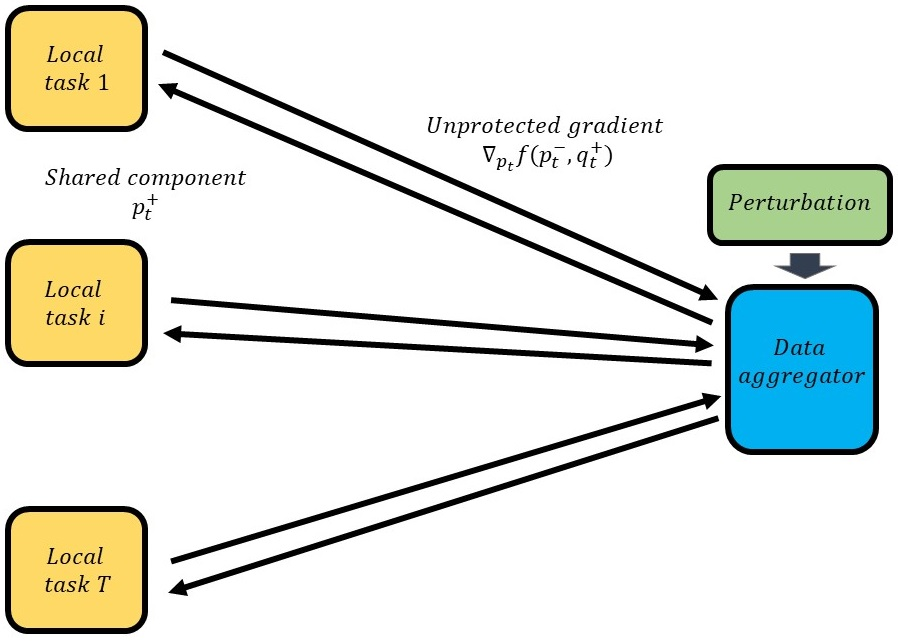
\includegraphics[scale=0.35]{figure/framework.jpg}
\caption{Proposed framework.}
\label{fig:framework} 
\end{figure}
